\documentclass{article}
\usepackage[utf8]{inputenc}
\usepackage{amsmath}
\usepackage{amssymb}
\usepackage{amsthm} %nodig voor blokje
\usepackage{marginnote}
\usepackage{graphicx}
\usepackage[margin=1in,footskip=0.25in]{geometry} %heb wat meer ruimte
\newcommand\header[1]{\framebox[\linewidth]{\textsc{Opgave #1}}\\}
\newcommand{\Z}{\mathbb{Z}}
\newcommand{\R}{\mathbb{R}}
\newcommand{\Q}{\mathbb{Q}}
\newcommand{\C}{\mathbb{C}}
\newcommand{\N}{\mathbb{N}}
\newcommand{\D}{\partial}
\begin{document}
\reversemarginpar
\section{Equilibrium}
\subsection{Basic model}
\marginnote{Definition} A board has reached \underline{equilibrium} after $g$ generations if in the $g+1$-th generation, no one has moved.\\
One of the research questions was: will the board reach an equilibrium (that is, no more moves)? Based on intuition, you'd expect this to be true. An individual who moves, does this to a place where there are relatively more neighbours of her type, so most of the time there are more individuals that gain happiness than those who lose happiness. In the basic model however, this is almost always true, but sometimes we get a periodic solution.\\
\textbf{Counterexample.} Consider the following board.
\begin{figure}[!ht]
\begin{center}
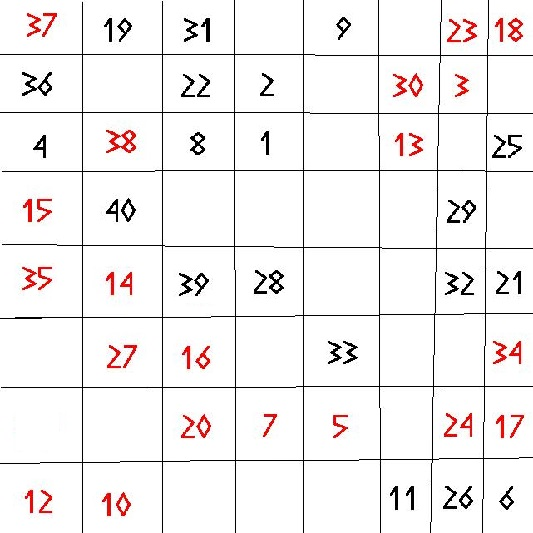
\includegraphics[scale=0.3]{segregation_tegenvb.jpg}
\end{center}
\caption{Counter example: 37 and 38 will move periodically.}\label{counterexample}
\end{figure}
The numbers stand for the turn order (1 is selected first, then 2, etc.). Red and black stand for the 2 types. After some checkwork, we see that individuals 1 to 36 are all happy, but 37 is not. In 37's turn, we see that 37 has a happiness of $0$, and the closest empty spot has happiness of $\frac{1}{7} > 0$, so 37 will move to this spot. New board:
\begin{figure}[!ht]
\begin{center}
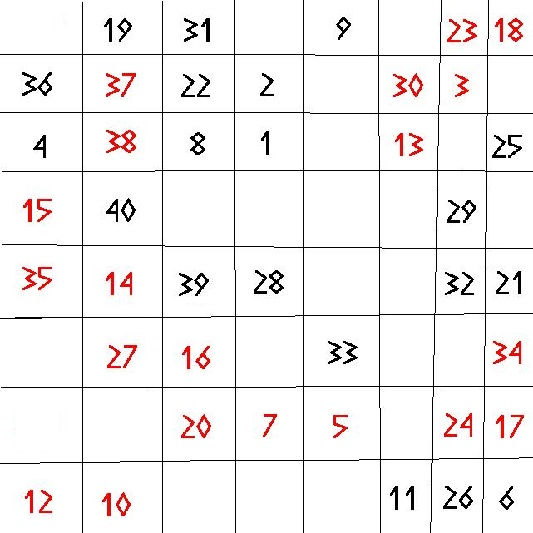
\includegraphics[scale=0.25]{segregation_tegenvb_1.jpg}
\end{center}
\caption{Counter example: 37 and 38 will move periodically.}\label{counterexample1}
\end{figure}
\\Next, it's 38's turn. 38 has a happiness of $\frac{2}{7}$. The closest spot with greater happiness is the nearby corner spot with happiness $\frac{1}{3}$. Now the board looks like this:\\
\begin{figure}[!ht]
\begin{center}
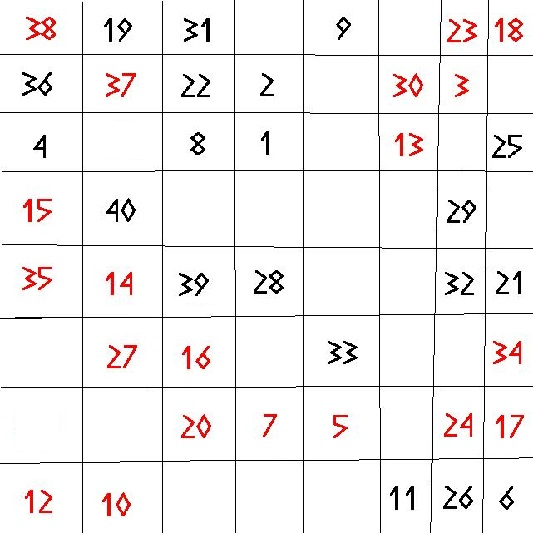
\includegraphics[scale=0.25]{segregation_tegenvb_2.jpg}
\end{center}
\caption{Counter example: 37 and 38 will move periodically.}\label{counterexample2}
\end{figure}
\\The others will remain happy and will not move. When it's 37's turn again, 37 has happiness $\frac{1}{7} < \frac{1}{3}$. The closest empty spot has happiness $\frac{1}{6} > \frac{1}{7}$, so 37 will move to that spot. Now 37 and 38 have swapped position:\\
\begin{figure}[!ht]
\begin{center}
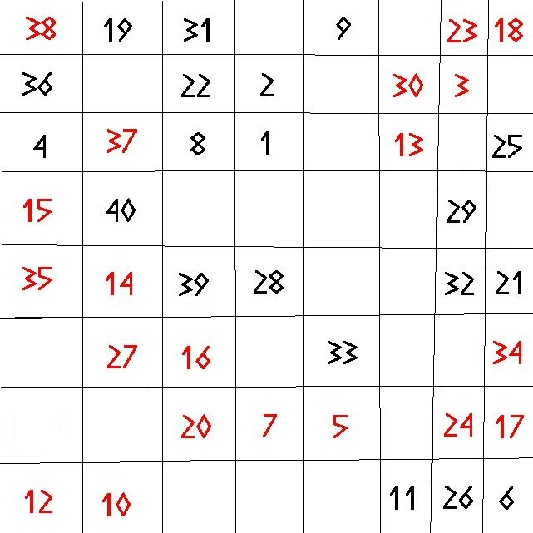
\includegraphics[scale=0.25]{segregation_tegenvb_3.jpg}
\end{center}
\caption{Counter example: 37 and 38 will move periodically.}\label{counterexample3}
\end{figure}
Since 37 and 38 are of the same type, those 3 moves will repeat: we have a periodic solution.\\
\textbf{Now what went wrong?} After the first move, both 37 and 38 will gain happiness, but on the third move, 38 will lose all of her happiness. We get an endless loop.\\
\newpage
\subsection{random displacement}
Now consider the situation that, when an individual is unhappy, she will move to a random empty spot (uniform distribution). In this situation, we always get an equilibrium, but we cannot say when.\\
\textbf{Theorem.} If, for a certain configuration of board size, number of people of each type and number of types, there exists a
\begin{proof}

\end{proof}
\end{document}